\documentclass{article}

\usepackage{fancyhdr}
\usepackage{extramarks}
\usepackage{amsmath}
\usepackage{amsthm}
\usepackage{amsfonts}
\usepackage{tikz}
\usepackage[plain]{algorithm}
\usepackage{algpseudocode}
\usepackage{pgfplots}
\usepackage{graphicx}

\usetikzlibrary{automata,positioning}

\graphicspath{ {./img} }

%
% Basic Document Settings
%

\topmargin=-0.45in
\evensidemargin=0in
\oddsidemargin=0in
\textwidth=6.5in
\textheight=9.0in
\headsep=0.25in

\linespread{1.1}

\pagestyle{fancy}
\lhead{\hmwkAuthorName}
\chead{\hmwkClass:\ \hmwkTitle}
\rhead{\firstxmark}
\lfoot{\lastxmark}
\cfoot{\thepage}

\renewcommand\headrulewidth{0.4pt}
\renewcommand\footrulewidth{0.4pt}

\setlength\parindent{0pt}
\setlength{\parskip}{5pt}

%
% Create Problem Sections
%

\newcommand{\enterProblemHeader}[1]{
    \nobreak\extramarks{}{Problem \arabic{#1} continued on next page\ldots}\nobreak{}
    \nobreak\extramarks{Problem \arabic{#1} (continued)}{Problem \arabic{#1} continued on next page\ldots}\nobreak{}
}

\newcommand{\exitProblemHeader}[1]{
    \nobreak\extramarks{Problem \arabic{#1} (continued)}{Problem \arabic{#1} continued on next page\ldots}\nobreak{}
    \stepcounter{#1}
    \nobreak\extramarks{Problem \arabic{#1}}{}\nobreak{}
}

\setcounter{secnumdepth}{0}
\newcounter{partCounter}
\newcounter{homeworkProblemCounter}
\setcounter{homeworkProblemCounter}{1}
\nobreak\extramarks{Problem \arabic{homeworkProblemCounter}}{}\nobreak{}

%
% Homework Problem Environment
%
% This environment takes an optional argument. When given, it will adjust the
% problem counter. This is useful for when the problems given for your
% assignment aren't sequential. See the last 3 problems of this template for an
% example.
%
\newenvironment{homeworkProblem}[1][-1]{
    \ifnum#1>0
        \setcounter{homeworkProblemCounter}{#1}
    \fi
    \section{Problem \arabic{homeworkProblemCounter}}
    \setcounter{partCounter}{1}
    \enterProblemHeader{homeworkProblemCounter}
}{
    \exitProblemHeader{homeworkProblemCounter}
}

%
% Homework Details
%   - Title
%   - Due date
%   - Class
%   - Section/Time
%   - Instructor
%   - Author
%

\newcommand{\hmwkTitle}{Homework\ \#2}
\newcommand{\hmwkDueDate}{October 30, 2023}
\newcommand{\hmwkClass}{ECE 271A}
\newcommand{\hmwkClassInstructor}{Professor Vasconcelos}
\newcommand{\hmwkAuthorName}{\textbf{Ray Tsai}}
\newcommand{\hmwkPID}{A16848188}

%
% Title Page
%

\title{
  \vspace{2in}
  \textmd{\textbf{\hmwkClass:\ \hmwkTitle}}\\
  \normalsize\vspace{0.1in}\small{Due\ on\ \hmwkDueDate\ at 11:59pm}\\
  \vspace{0.1in}\large{\textit{\hmwkClassInstructor}} \\
  \vspace{3in}
}

\author{
  \hmwkAuthorName \\
  \vspace{0.1in}\small\hmwkPID
}
\date{}

\renewcommand{\part}[1]{\textbf{\large Part \Alph{partCounter}}\stepcounter{partCounter}\\}

%
% Various Helper Commands
%

% Useful for algorithms
\newcommand{\alg}[1]{\textsc{\bfseries \footnotesize #1}}

% For derivatives
\newcommand{\deriv}[1]{\frac{\mathrm{d}}{\mathrm{d}x} (#1)}

% For partial derivatives
\newcommand{\pderiv}[2]{\frac{\partial}{\partial #1} (#2)}

% Integral dx
\newcommand{\dx}{\mathrm{d}x}

% Probability commands: Expectation, Variance, Covariance, Bias
\newcommand{\Var}{\mathrm{Var}}
\newcommand{\Cov}{\mathrm{Cov}}
\newcommand{\Bias}{\mathrm{Bias}}
\newcommand*{\Z}{\mathbb{Z}}
\newcommand*{\Q}{\mathbb{Q}}
\newcommand*{\R}{\mathbb{R}}
\newcommand*{\C}{\mathbb{C}}
\newcommand*{\N}{\mathbb{N}}
\newcommand*{\prob}{\mathds{P}}
\newcommand*{\E}{\mathds{E}}

\begin{document}

\maketitle

\pagebreak

\begin{homeworkProblem}
  Let $p(x|\omega_i) \sim N(\mu_i, \Sigma)$ for a two-catagory d-dimensional problem with the same covariances but arbitrary means and prior probabilities. 
  Consider the squared Mahalanobis distance
  \[
    r^2_i = (x - \mu_i)^T\Sigma^{-1}(x - \mu_i).
  \]

  \part{A}

  Show that the gradient of $r^2_i$ is given by
  \[
    \nabla r^2_i = 2\Sigma^{-1}(x - \mu_i).
  \]

  \textbf{Solution}

  Notice that
  \begin{align*}
    r^2_i 
    &= (x - \mu_i)^T\Sigma^{-1}(x - \mu_i) \\
    &= x^T\Sigma^{-1}x - 2\mu^T\Sigma^{-1}x + \mu_i^T\Sigma^{-1}\mu_i \\
    &= \sum_k\sum_j \Sigma^{-1}_{kj}x_kx_j - 2\sum_k\sum_j \Sigma^{-1}_{kj}\mu_{i_k}x_j + \sum_k\sum_j \Sigma^{-1}_{kj}\mu_{i_k}\mu_{i_j}.
  \end{align*}
  Thus,
  \begin{align*}
    \frac{\partial r^2_i}{\partial x_m} 
    &= \frac{\partial}{\partial x_m} \left(\sum_k\sum_j \Sigma^{-1}_{kj}x_kx_j - 2\sum_k\sum_j \Sigma^{-1}_{kj}\mu_{i_k}x_j + \sum_k\sum_j \Sigma^{-1}_{kj}\mu_{i_k}\mu_{i_j}\right) \\
    &= \frac{\partial}{\partial x_m} \left(\sum_k\sum_j \Sigma^{-1}_{kj}x_kx_j\right)  - 2\sum_k \Sigma^{-1}_{km}\mu_{i_k} \\
    &= \frac{\partial}{\partial x_m} \left(\Sigma^{-1}_{mm}x_m^2 + \sum_{k \neq m} \Sigma^{-1}_{km}x_kx_m + \sum_{j \neq m} \Sigma^{-1}_{mj}x_mx_j + \sum_{k \neq m}\sum_{j \neq m} \Sigma^{-1}_{kj}x_kx_j\right)  - 2\sum_k \Sigma^{-1}_{km}\mu_{i_k} \\
    &= 2\Sigma^{-1}_{mm}x_m + \sum_{k \neq m} \Sigma^{-1}_{km}x_k + \sum_{j \neq m} \Sigma^{-1}_{mj}x_j - 2\sum_k \Sigma^{-1}_{km}\mu_{i_k} \\
    &= \sum_{k} \Sigma^{-1}_{km}x_k + \sum_{j} \Sigma^{-1}_{mj}x_j - 2\sum_k \Sigma^{-1}_{km}\mu_{i_k} \\
    &= 2\sum_{k} \Sigma^{-1}_{mk}(x_k - \mu_{i_k}).
  \end{align*}
  Notice that $\frac{\partial r^2_i}{\partial x_m}$ is simply dot product of the $m$-th row of $\Sigma^{-1}$ and $(x - \mu)$ times $2$, and so $\nabla r^2_i = 2\Sigma^{-1}(x - \mu_i)$.
\end{homeworkProblem}

\part{B}

Show that at any position on a given line through $\mu_i$ the gradient $\nabla r_i^2$ points in the same direction.
Must this direction be parellel to that line?
\\

\textbf{Solution}

Let $L = \{ax + \mu_i \, | \, a \in \R\}$, for some $x \in \R^d$. Let $y = lx + \mu_i \in L$. 
Then, $\nabla^2_i r(y) = \nabla r^2_i = 2\Sigma^{-1}(y - \mu_i) = 2l\Sigma^{-1}x$, and so $\nabla r_i^2$ is not parellel to the line $L$ unless $\Sigma^{-1} = \Sigma = I$.

\part{C}

Show that $\nabla r^2_1$ and $\nabla r^2_2$ point in opposite directions along the line from $\mu_1$ to $\mu_2$.
\\

\textbf{Solution}

Let $p = a\mu_1 + (1 - a)\mu_2$ be a point on the line from $\mu_1$ to $\mu_2$, for $a \in [0, 1]$. 
Then,
\begin{gather}
  \nabla r^2_1(p) = 2\Sigma^{-1}(p - \mu_1) = 2(a - 1)\Sigma^{-1}(\mu_1 - \mu_2) \\
  \nabla r^2_2(p) = 2\Sigma^{-1}(p - \mu_2) = 2a\Sigma^{-1}(\mu_1 - \mu_2).
\end{gather}
When $a = 0$ or $1$, $a$ or $a - 1$ become $0$.
When $a \in (0, 1)$, $a$ and $a - 1$ has opposite signs.
Thus, we conclude that $\nabla r^2_1(p)$ and $\nabla r^2_2(p)$ points toward opposite directions.
\\

\part{D}

Show that the optimal separating hyperplane is tangent to the constant probability density hyperellipsoids at the point that the separating hyperplane cuts the line from $\mu_1$ to $\mu_2$.
\\

\textbf{Solution}

We know the optimal decision rule is $i^*(x) = \underset{i}{\arg \max} \ln P_{X|Y}(x|i) + \ln P_Y(i)$.
Assume that $P_{X|Y}(x|i)$ is some Gaussian distribution with mean $\mu_i$ and covariance matrix $\Sigma$, denoted as $G(x, \mu_i, \Sigma)$.
Then, our decision rule becomes 
\begin{align*}
  i^*(x) 
  &= \underset{i}{\arg \max} \, -\frac{1}{2}(x - \mu_i)^T\Sigma^{-1}(x - \mu_i) + \ln P_Y(i) \\
  &= \underset{i}{\arg \max} \, \mu_i^T\Sigma^{-1} x - \frac{1}{2}\mu_i^T\Sigma^{-1}\mu_i + \ln P_Y(i).
\end{align*}
Let $w_i = \mu_i^T\Sigma^{-1}$ and $w_{i0} = -\frac{1}{2}\mu_i^T\Sigma^{-1}\mu_i + \ln P_Y(i)$.
Thus, the optimal decision place between class $1$ and $2$ is
\begin{align*}
  \mu_1^T\Sigma^{-1} x + w_{i1} - \mu_1^T\Sigma^{-2} x - w_{i2}
  &= (\Sigma^{-1}(\mu_1 - \mu_2))^T x + (w_{i1} - w_{i2}) = 0.
\end{align*}
Let $p$ be a point on the line from $\mu_1$ to $\mu_2$ where the decision plane cuts through.
From part C, we know that $\nabla r^2_1(p) = 2(a - 1)\Sigma^{-1}(\mu_1 - \mu_2)$ and $\nabla r^2_2(p) = 2a\Sigma^{-1}(\mu_1 - \mu_2)$.
Notice that the direction of the plane $\Sigma^{-1}(\mu_1 - \mu_2)$ is parallel to both $\nabla r^2_1(p)$ and $\nabla r^2_1(p)$, which implies that the plane is orthogonal to the gradients at point $p$.
Since gradients of a function are also orthogonal to the constant contours of its function, we thus know that the optimal decision plane is tangent to the constant probability density function hyperellipsoids at point $p$.
\\

\part{E}

True or False: For a two-catagory problem involving normal densities with arbitrary means and covariances, and $P_Y(w_1) = P_Y(w_2) = \frac{1}{2}$, the Bayes decision boundary consists of the set of points of equal Mahalanobis distance from the respective sample means.
\\

\textbf{Solution}

False. Although the decision boundary consists of the points of equal Mahalanobis distance from the two class means in this case, we cannot guarantee the sample means equal the "true" class means.


\pagebreak

\begin{homeworkProblem}
  In this problem we will consider the ML estimate of the parameters of a multinomial distribution.
  Consider a random variable $X$ such that $P_X(k) = \pi_k, k \in \{1, \dots, N\}$. Suppose we draw n independent
  observations from $X$ and form a random vector $C = (C_1, . . . , C_N)^T$,
  where $C_k$ is the number of times
  that the observed value is $k$ (i.e. $C$ is the histogram of the sample of observations). 
  Then, $C$ has multinomial distribution
  \[
    P_{C_1,\dots,C_N}(c_1,\dots,c_N) = \frac{n!}{\prod_{k = 1}^N c_k!}\prod^N_{j = 1}\pi^{c_j}_j.
  \]

  \part{A}

  Derive the ML estimator for the parameters $\pi_i$, $i = 1, \dots , N$.
  \\

  \textbf{Solution}

  We first take the logarithm of $P_{C_1,\dots,C_N}(c_1,\dots,c_N)$ and get
  \[
    \ln P_{C_1,\dots,C_N}(c_1,\dots,c_N) = \ln \frac{n!}{\prod_{k = 1}^N c_k!} + \sum^N_{j = 1} c_j \ln \pi_j.
  \]
  Let $\theta = (\pi_1, \dots, \pi_N)^T$, and let $L(\theta, \lambda) = \ln P_{C_1,\dots,C_N}(c_1,\dots,c_N) + \lambda\left(\sum^N_j \pi_j - 1\right)$.
  Then,
  \begin{gather*}
    \nabla_{\theta}L = \left(\frac{c_1}{\pi_1},\dots, \frac{c_N}{\pi_N}\right)^T + (\lambda, \dots, \lambda)^T = 0 \\
    \frac{\partial}{\partial \lambda}L = \sum_{j = 1}^N \pi_j - 1 = 0.
  \end{gather*}
  For $1 \leq j \leq N$, we get $\frac{c_j}{\pi_j} + \lambda = 0$, and so $c_j + \pi_j\lambda = 0$. 
  Then, $\sum^N_{j = 1} (c_j + \pi_j\lambda) = n + \lambda = 0$, and thus $ \lambda = -n$. 
  We also take the Hessian of $L$. Notice that 
  \[
      \frac{\partial^2 L}{\partial \pi_i \partial \pi_j} = \begin{cases}
          -\frac{c_j}{\pi_j^2}, & i = j \\
          0, & i \neq j
      \end{cases},
  \]
  and so $\nabla^2_{\theta} L = \text{diag}\left(-\frac{c_i}{\pi_i^2}, \dots, -\frac{c_N}{\pi_N^2}\right)$.
  Since the Hessian of $L$ is obviously negative definite, the critical point we are looking for is indeed a maximum point.
  Therefore, we obtain the ML estamator $\hat{\theta} = \left(\frac{C_1}{n},\dots, \frac{C_N}{n}\right)$.
  \\

  \part{B}

  Is the estimator derived in part A unbiased? 
  What is its variance? 
  Is this a good estimator? 
  Why?
  \\

  \textbf{Solution}
  Since 
  \begin{align*}
    Bias(\hat{\pi_j})
    &= E[\hat{\pi_j} - \pi_j] \\
    &= \frac{1}{n}E[C_j] - \pi_j \\
    &= \frac{1}{n} \cdot n\pi_j - \pi_j = 0,
  \end{align*}
  $\hat{\theta}$ is unbiased.

  We also know
  \begin{align*}
    Var(\hat{\pi_j}) 
    &= \frac{1}{n^2}Var(C_j) = \frac{\pi_j(1 - \pi_j)}{n}.
  \end{align*}
  This shows that our estimator converges to the perfect estimation as we increase our sample size, as thus $\hat{\theta}$ is a good estimator.
\end{homeworkProblem}

\pagebreak

\begin{homeworkProblem}
  Consider an extreme case of the general issue discussed in Problem $7$, one in which it is possible that the maximum likelihood solution leads to the worst possible classifier, i.e., one with an error that approaches $100\%$.
  Suppose our data in fact comes from two one-dimensional distribution of the forms 
  \begin{gather}
    p(x|\omega_1) \sim [(1 - k)\delta(x - 1) + k\delta(x + X)] \\
    p(x|\omega_2) \sim [(1 - k)\delta(x + 1) + k\delta(x - X)],
  \end{gather}
  where $X$ is positive, $0 \leq k < 0.5$ represents the portion of the total probability mass concentrated at the point $\pm X$,
  and $\delta(.)$ is the Dirac delta function.
  Suppose our poor models are of the form $p(x|\omega_1,\mu_1) \sim N(\mu_1, \sigma^2_1)$, and $p(x|\omega_2,\mu_2) \sim N(\mu_2, \sigma^2_2)$ and we form a maximum likelihood classifier.
  \\

  \part{A}

  Consider the symmetries in the problem and show that in the infinite data case the decision boundary will always be at $x = 0$, regardless of $k$ and $X$.
  \\

  \textbf{Solution}

  We first calculate the means and variances of $p(x|\omega_1)$ and $p(x|\omega_2)$ and get
  \begin{gather}
    \mu_1 = (1 - k) - kX \\
    \mu_2 = kX - (1 - k) \\
    \sigma_1^2 = (1 - k)(\mu_1 - 1)^2 + k(\mu_1 + X)^2 \\
    \sigma_2^2 = (1 - k)(\mu_2 + 1)^2 + k(\mu_2 - X)^2.
  \end{gather}
  Notice that $\sigma_2^2 = \sigma_1^2 = \sigma^2$, as $\mu_1 = -\mu_2$.
  In the infinite data case, the sample means and variances converges to the the theoretic mean of our model,
  and so the decision boundary is
  \[
    x = \frac{\mu_1 + \mu_2}{2} - \frac{\sigma^2}{\mu_2 - \mu_1}\ln\frac{P_Y(\omega_1)}{P_Y(\omega_2)} = 0.
  \]

  \part{B}

  Recall that the maximum likelihood estimate of either mean, $\hat{\mu_i}$, is the mean of its distribution.
  For a fixed $k$, find the value of $X$ such that the maximum likelihood estimates of the means "switch," i.e., where $\hat{\mu_1} \geq \hat{\mu_2}$.
  \\

  \textbf{Solution}
  \begin{align*}
    \hat{\mu_1} &\geq \hat{\mu_2} = -\hat{\mu_1} \\
    \hat{\mu_1} &\geq 0 \\
    (1 - k) - kX &\geq 0 \\
    \frac{1 - k}{k} &\geq X.
  \end{align*}
  Thus, the means "switch" when $X = \frac{1 - k}{k}$.
  \\

  \part{C}

  Plot the true distributions and the Gaussian estimates for the particular case
  $k = .2$ and $X = 5$ What is the classification error in this case?
  \\

  \textbf{Solution}

  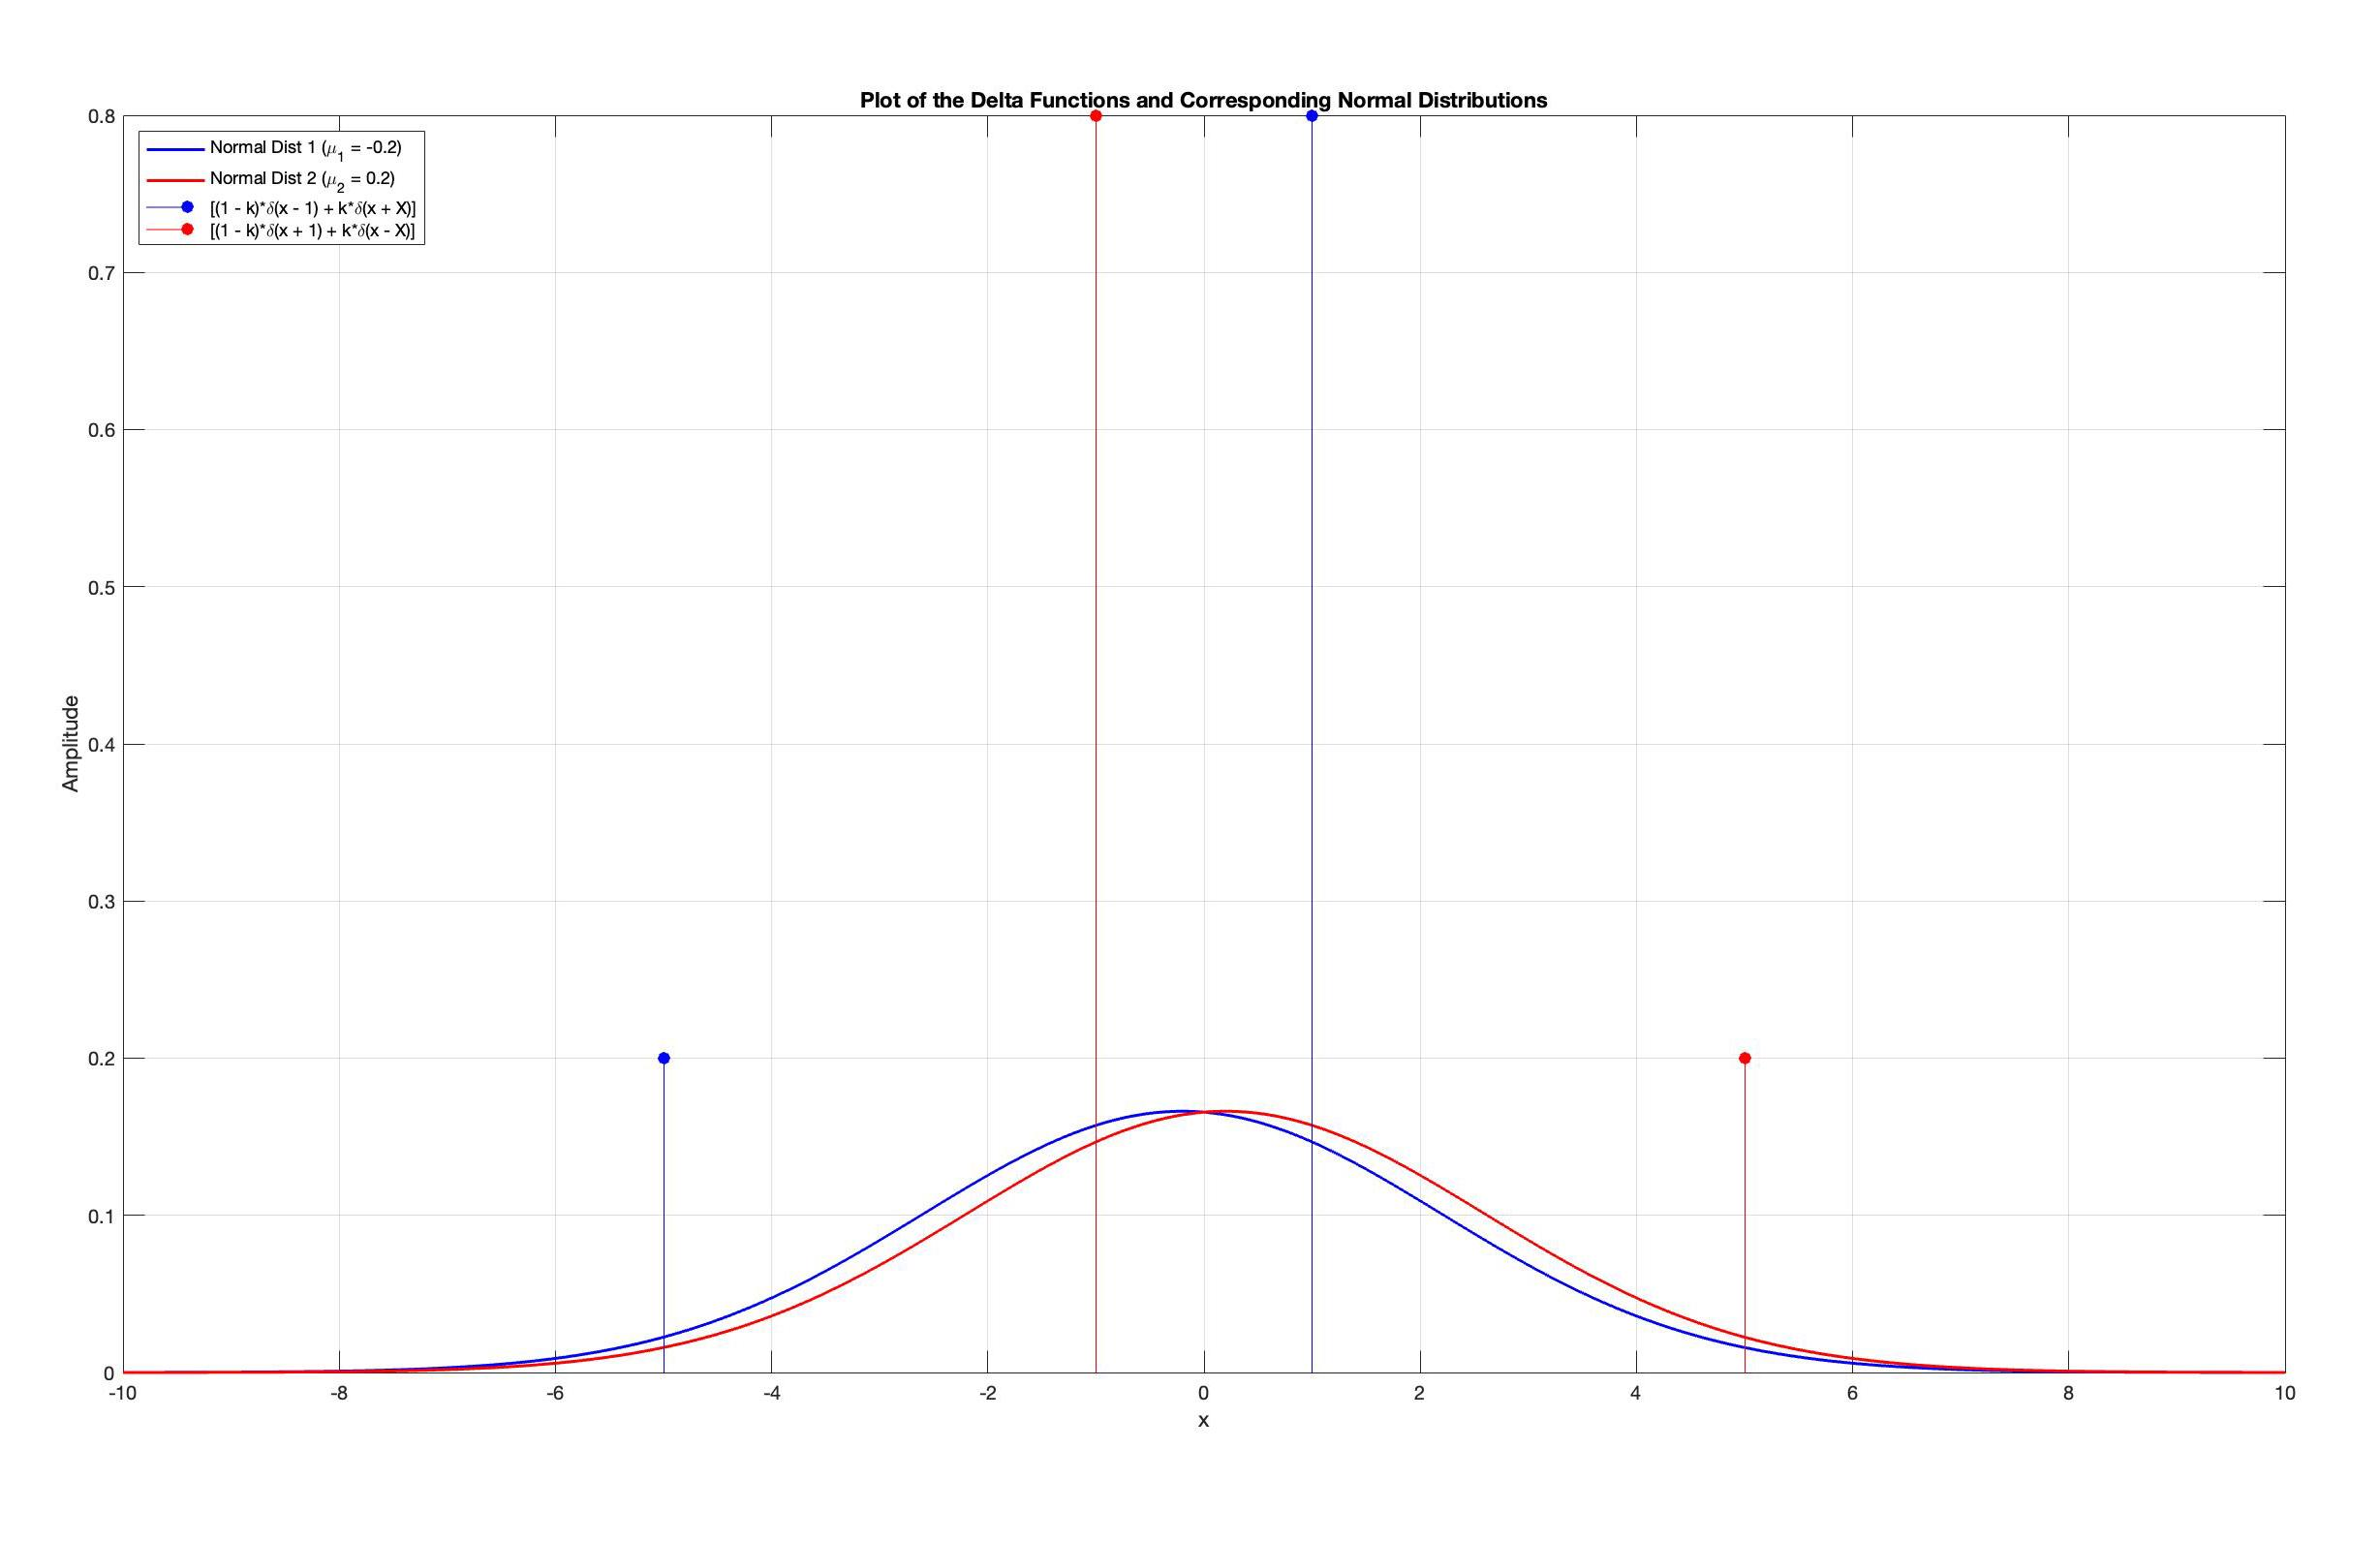
\includegraphics[width=\textwidth]{Q3c}

  The error is 
  \begin{align*}
    P_{X,Y}(i(x) \neq y)
    &= P_{X|Y}(i(x) = 1 | y = 2)P_Y(2) + P_{X|Y}(i(x) = 2 | y = 1)P_Y(1) \\
    &= P_{X|Y}(x \leq 0 | y = 2)P_Y(2) + P_{X|Y}(x \geq 0 | y = 1)P_Y(1) \\
    &= P_{X|Y}(x \leq 0 | y = 2)(P_Y(1) + P_Y(2)) \\
    &= P_{X|Y}(x \leq 0 | y = 2) \\
    &= 1 - k = 0.8.
  \end{align*}

  \part{D}

  Find a dependence $X(k)$ which will guarantee that the estimated mean $\hat{\mu_1}$ of
  $p(x|\omega_1)$ is less than zero. (By symmetry, this will also insure $\hat{\mu_2} > 0$.)
  \\

  \textbf{Solution}

  Consider $X = \frac{1}{k}$. Since, $\hat{\mu_1} = (1 - k) - kX = -k < 0$, $X$ meets the requirements.
  
  \pagebreak

  \part{E}

  Given your $X(k)$ just derived, state the classification error in terms of $k$
  \\

  \textbf{Solution}

  Did it in part C already bruh. $1 - k$.
  \\

  \part{F}

  Suppose we constrained our model space such that $\sigma^2_1 = \sigma^2_2 = 1$ (or indeed any other constant). Would that change the above results?
  \\

  \textbf{Solution}

  No. The decision boundary would not change unless $\sigma_1^2 \neq \sigma_2^2$, and thus the classification error would also not be affected.
  \\

  \part{G}

  Discuss how if our model is wrong (here, does not include the delta functions),
  the error can approaches $100\%$ (in probability). Does this surprising answer
  arise because we have found some local minimum in parameter space?
  \\

  \textbf{Solution}

  Consider $k \rightarrow 0$. Then, according to the result we concluded in part E, the classification error approaches $100\%$.
  This is not due to finding the local minimum but simply a class classification mismatch.

\end{homeworkProblem}

\pagebreak

\begin{homeworkProblem}
  Suppose we employ a novel method for estimating the mean of a data set
  $\mathcal{D} = \{x_1, x_2, \dots, x_n\}$: we assign the mean to be the value of the first point in the set,
  i.e., $x_1$.
  \\

  \part{A}

  Show that this method is unbiased.
  \\

  \textbf{Solution}

  Suppose that $\hat{\mu} = x_1$. Then, $Bias(\hat{\mu}) = E[\hat{\mu} - \mu] = E[x_1] - \mu = \mu - \mu = 0$, and thus $\hat{\mu}$ is unbiased.
  \\

  \part{B}

  State why this method is nevertheless highly undesirable.
  \\

  \textbf{Solution}

  We check the variance of this estimator. Since
  \begin{align*}
    Var(\hat{\mu})
    &= Var(x_1),
  \end{align*}
  the variance of the estimator does not decrease even if we increase the sample size, and so $\hat{\mu}$ is not a good estimator.
\end{homeworkProblem}

\pagebreak

\begin{homeworkProblem}
  Let $p(x|\Sigma) \sim N(\mu, \Sigma)$ where $\mu$ is known and $\Sigma$ is unknown. Show that the
  maximum likelihood estimate for $\Sigma$ is given by
  \[
    \hat{\Sigma} = \frac{1}{n}\sum^n_{k = 1} (x_k - \mu)(x_k - \mu)^T
  \]
  by carrying out the following argument:
  \\

  \part{A}

  Prove the matrix identity $a^TAa = tr[Aaa^T]$, where the trace, $tr[A]$, is the sum
  of the diagonal elements of $A$.
  \\

  \textbf{Solution}

  On the RHS, we get $a^TAa = \sum_i\sum_j A_{ij}a_ia_j$. On the LHS, we get
  \begin{align*}
    tr[Aaa^T]
    &= \sum_i (Aaa^T)_{ii} \\
    &= \sum_i A_{i\cdot} (aa^T)_{\cdot i} \\
    &= \sum_i \sum_j A_{ij} (aa^T)_{ji} \\
    &= \sum_i \sum_j A_{ij} a_ia_j.
  \end{align*}
  Thus, we know $a^TAa = \sum_i\sum_j A_{ij}a_ia_j = tr[Aaa^T]$.
  \\

  \part{B}

  Show that the likelihood function can be written in the form
  \[
    p(x_1, \dots , x_n|\Sigma) = \frac{1}{\left((2\pi)^d|\Sigma|\right)^{\frac{n}{2}}} \exp \left[-\frac{1}{2}\text{tr}\left[\Sigma^{-1}\sum_{k = 1}^n(x_k - \mu)(x_k - \mu)^T\right]\right].
  \]

  \textbf{Solution}

  \begin{align*}
    p(x_1, \dots , x_n|\Sigma)
    &= \prod_{k = 1}^n\frac{1}{\left((2\pi)^d|\Sigma|\right)^{\frac{n}{2}}} \exp \left[-\frac{1}{2}(x_k - \mu)^T\Sigma^{-1}(x_k - \mu)\right] \\
    &= \frac{1}{\left((2\pi)^d|\Sigma|\right)^{\frac{n}{2}}} \exp \left[-\frac{1}{2}\sum_{k = 1}^n(x_k - \mu)^T\Sigma^{-1}(x_k - \mu)\right] \\
    &= \frac{1}{\left((2\pi)^d|\Sigma|\right)^{\frac{n}{2}}} \exp \left[-\frac{1}{2}\sum_{k = 1}^n\text{tr}\left[\Sigma^{-1}(x_k - \mu)(x_k - \mu)^T\right]\right] \\
    &= \frac{1}{\left((2\pi)^d|\Sigma|\right)^{\frac{n}{2}}} \exp \left[-\frac{1}{2}\text{tr}\left[\Sigma^{-1}\sum_{k = 1}^n(x_k - \mu)(x_k - \mu)^T\right]\right].
  \end{align*}

  \part{C}

  Let A = $\Sigma^{-1}\hat{\Sigma}$ and $\lambda_1, \dots, \lambda_n$ be the eigenvalues of $A$. Show that your result above leads to
  \[
    p(x_1, \dots , x_n|\Sigma) = \left(\frac{\prod_{k = 1}^d \lambda_k}{(2\pi)^d|\hat{\Sigma|}}\right)^{\frac{n}{2}} \exp \left[-\frac{n}{2}(\lambda_1 + \dots + \lambda_d)\right].
  \]

  \textbf{Solution}

  Since $|A| = \prod_{k = 1}^d \lambda_k$ and tr$(A) = \sum_{k = 1}^n \lambda^k$,
  \begin{align*}
    p(x_1, \dots , x_n|\Sigma) 
    &= \frac{1}{\left((2\pi)^d|\Sigma|\right)^{\frac{n}{2}}} \exp \left[-\frac{1}{2}\text{tr}\left[\Sigma^{-1}\sum_{k = 1}^n(x_k - \mu)(x_k - \mu)^T\right]\right] \\
    &= \left(\frac{|A\hat{\Sigma}^{-1}|}{(2\pi)^d}\right)^{\frac{n}{2}} \exp \left[-\frac{1}{2}\text{tr}\left[n\Sigma^{-1}\hat{\Sigma}\right]\right] \\
    &= \left(\frac{\prod_{k = 1}^d \lambda_k}{(2\pi)^d|\hat{\Sigma}|}\right)^{\frac{n}{2}} \exp \left[-\frac{n}{2}(\lambda_1 + \dots + \lambda_d)\right].
  \end{align*}

  \part{D}

  Complete the proof by showing that the likelihood is maximized by the choice
  $\lambda_1 = \dots = \lambda_d = 1$. 
  \\

  \textbf{Solution}

  Let $\lambda = (\lambda_1, \dots, \lambda_d)^{T}$
  \begin{align*}
    g(x_1, \dots, x_n|\lambda) 
    &= \ln p(x_1, \dots , x_n|\Sigma) \\
    &= \frac{n}{2}\sum_{k = 1}^d \ln \lambda_k - \frac{dn}{2}\ln 2\pi - \frac{n}{2} \ln |\hat{\Sigma}| - \frac{n}{2} \sum_{i = 1}^d \lambda_i \\
    &= \frac{n}{2}\left[\sum_{k = 1}^n \ln (\lambda_k) - \lambda_k \right] - \frac{n}{2}\left[d\ln 2\pi - \ln |\hat{\Sigma}|\right].
  \end{align*}
  Then,
  \[
    \nabla_{\lambda} g = \frac{n}{2}\begin{bmatrix}
      \lambda_1^{-1} - 1 \\
      \vdots \\
      \lambda_d^{-1} - 1
    \end{bmatrix} = 0,
  \]
  and so the $\lambda = (1, \dots, 1)^T$ is a critical point. We now take the Hessian of $g$. Notice that
  \[
    \frac{\partial^2 g}{\partial \lambda_i\lambda_j} = \begin{cases}
      -\lambda_i^{-2} & i = j \\
      0 & i \neq j
    \end{cases},
  \]
  and so $\nabla^2_{\lambda} = \text{diag}(-\lambda_1^{-2}, \dots, -\lambda_d^{-2})$, which is obviously negative definite.
  The likelihood is indeed maximized by the choice $\lambda = (1, \dots, 1)^T$.
  It immediately follows that $A = \Sigma^{-1}\hat{\Sigma} = I$, so $\Sigma = \hat{\Sigma}$, and we are done.
\end{homeworkProblem}
  
\end{document}